\documentclass[a4paper]{article}

\usepackage{amsmath}
\usepackage{array}
\usepackage[toc,page]{appendix}
\usepackage{pdfpages}
\usepackage[utf8]{inputenc}
\usepackage{csquotes}
\usepackage[style=apa,sortcites=true,sorting=nyt]{biblatex}
\usepackage[hidelinks]{hyperref}
\hypersetup{colorlinks=False}
\usepackage{pdfpages}
\usepackage{xcolor}
\definecolor{mygray}{rgb}{0.8,0.8,0.8}
\usepackage{realboxes}
\usepackage[nottoc]{tocbibind}

\usepackage{titlesec}
\setcounter{secnumdepth}{4}

\usepackage{float}
% \usepackage{color} maybe do this another time
\usepackage{listings}
\lstset{
	language=[11]C++,
	numbers=left,
	stepnumber=1,
	showstringspaces=false
	showtabs=false,
	keepspaces,
	frame=tb,
}

%\usepackage{parskip} 
%\setlength{\parskip}{12pt}

\usepackage{graphicx}
\graphicspath{{./images/}}

\addbibresource{dissertation.bib}
\DeclareLanguageMapping{american}{american-apa}

\usepackage[toc,nopostdot, automake,acronym]{glossaries-extra}
\makeglossaries
%\renewcommand{\glsgroupskip}{}
\RestoreAcronyms
\setcounter{tocdepth}{4}
\renewcommand{\glsgroupskip}{}
%\renewcommand{\glsnamefont}[1]{\makefirstuc{#1}}

% glossary entries
% Look at web-dev business proposal for this...

% glossary entries
			\newglossaryentry{compilerg}{name={Compiler},
                text = {compiler},
				plural={compilers}, description={A program which translates code (plain text) into assembly code. Examples include GCC and Clang.}}

			\newglossaryentry{interpreterg}{name={Interpreter},
                text = {interpreter},
				plural={interpreters}, description={Translates the code to line by line, during execution (such as with Python and Javascript)}}


			\newglossaryentry{assemblerg}{name={Assembler},
                text = {interpreter},
				plural={assemblers}, description={Translates assembly code into machine code (binary).}}


			%working
			\newglossaryentry{gcg}{name={Garbage Collector},
				description={(\gls{gca}) A program or part of a program which automatically frees unused (garbage) memory during runtime - increases overhead for the program.}}
			\newacronym{gca}{GC}{\gls{gcg}}

			\newglossaryentry{bstg}{name={Binary Search Tree},
				description={(\gls{bsta}) A sorted, recursive data structure which has a root node, and separates all values less than the root node into one half, and all values greater than the root node into the other half.}}

			\newacronym{bsta}{BST}{\gls{bstg}}

			\newglossaryentry{raiig}{name={Resource Acquisition is Initialisation},
				description={(\gls{raiia}) is a C++ idiom, relating to object lifetimes relating to the scope they're declared in, and having an object's constructor / destructor completely deal with funcitonality of an object's lifetime beginning / ending (respectively), such as acquiring / freeing all associated memory.}}
			\newacronym{raiia}{RAII}{\gls{raiig}}

			\newglossaryentry{llvmg}{name={Low Level Virtual Machine},
            description={(\gls{llvma}) -  ``\emph{The LLVM Project is a collection of modular and reusable compiler and toolchain technologies.}'' \parencite{what-is-llvm}. LLVM allows developers to write a front-end for any programming language which can then be compiled to LLVM's ``language independent intermediate representation'' which can then be compiled to portable, optimisable machine code by LLVM's backend.}}
			\newacronym{llvma}{LLVM}{\gls{llvmg}}

			\newglossaryentry{ubg}{name={Undefined Behaviour},
            description={(\gls{uba}) - Behaviour which cannot be formally described by the C++ standard. Undefined behaviour can be caused by a program being ill-formed, data-races, etc \parencite{cpp-reference-ub}.}}
			\newacronym{uba}{UB}{\gls{ubg}}

			\newglossaryentry{abig}{name={Application Binary Interface},
            description={(\gls{abia}) - Defines the rules by which different binary programs which are compiled separately can interoperate. \gls{abia} is a topic of controversy in the C++ community as the standards community are often criticised for maintaining backwards \gls{abia} compatibility at the expense of deverloping the language further \parencite{cpp-abi}.}}
			\newacronym{abia}{ABI}{\gls{abig}}

			\newglossaryentry{gccg}{name={GNU Compiler Collection},
            description={(\gls{gcca}) - A set of compilers for various languages developed by the GNU project (an open source foundation, responsible for the GNU General Purpose software license, emacs, large components of the GNU / Linux operating system, etc).}}
			\newacronym{gcca}{GCC}{\gls{gccg}}

			\newglossaryentry{msvcg}{name={Microsoft Visual C++},
            description={(\gls{msvca}) - Microsoft's compiler for C++}}
			\newacronym{msvca}{MSVC}{\gls{msvcg}}
\begin{document}

\begin{titlepage}
    \begin{center}
        \vspace*{1cm}
            
        \Huge
        \textbf{A Partial Runtime Implementation of the ``Rust Borrow Checker'' In C++}
            
        \vspace{0.5cm}
        \LARGE
%        Thesis Subtitle
            
        \vspace{1.5cm}
            
        \textbf{Fred Cook - 8463955}\\
        Supervised by: Olalekan Lanihun \& Carey Pridgeon
            
        \vfill
            
        \vspace{0.8cm}
            
        
\includegraphics[width=0.4\textwidth]{assets/coventry-university-logo.png}
            
        \Large
        Computer Science\\
        Faculty of Engineering, Environment, and Computing\\
        Coventry University\\
        2022-19-04
            
    \end{center}

%title
%author
%student id
%degree title
%supervisor name
%institution name
%coventry uni
%date of submission
    \pagenumbering{roman}
    \newpage
    \begin{abstract}
        C++ has been and is one of the most widely used programming languages in the industry, however, a common criticism is that C++ is ``unsafe'', meaning that it is susceptible to errors (primarily relating to memory) which lead to ``undefined behaviour'', security issues, and stability problems. Rust is a new programming language that aims to be similar to C++ in many ways but with the aforementioned issues rectified. The primary way Rust does this is through the usage of the ``Borrow Checker''.

        \begin{itemize}
            \item        The aim of this paper is to answer the following question: ``Is it possible to enforce some of (or potentially all) the rules and guarantees of the Rust Borrow Checker in C++?''
            \item        This dissertation provides a partial runtime implementation of the borrow checker in C++ in order to get improved memory safety in C++, therefore allowing developers to utilise mature libraries, learning resources, etc which Rust lacks to the same degree as C++.
            \item        The motivation for this paper is to be able to improve C++ as a language by improving it's memory safety and concurrency capabilities (eliminating data race scenarios), it's audience is therefore C++ developers aiming to improve the safety of their codebase(s).
            \item        The method is comprised of a series of test harnesses, used to demonstrate the ``correctness'' of different programs in the two respective languages, and the effects that this project has on C++ programs' behaviours.
            \item        This project is successful in replicating some of the behaviours of the borrow checker in C++, however, this is at the cost of having a larger runtime overhead (which the Rust implementation does not have), which is often highly undesirable in C++ programs due to the high performance needs of these programs.
            \item        The need for this paper is evidenced by the fact that other groups are working to bring more safety features (like those seen in Rust) to C++ as shown by \gls{llvma} \parencite{lifetime-annotations-cpp}.
\end{itemize}
    \end{abstract}
\end{titlepage}
\raggedbottom
\newpage

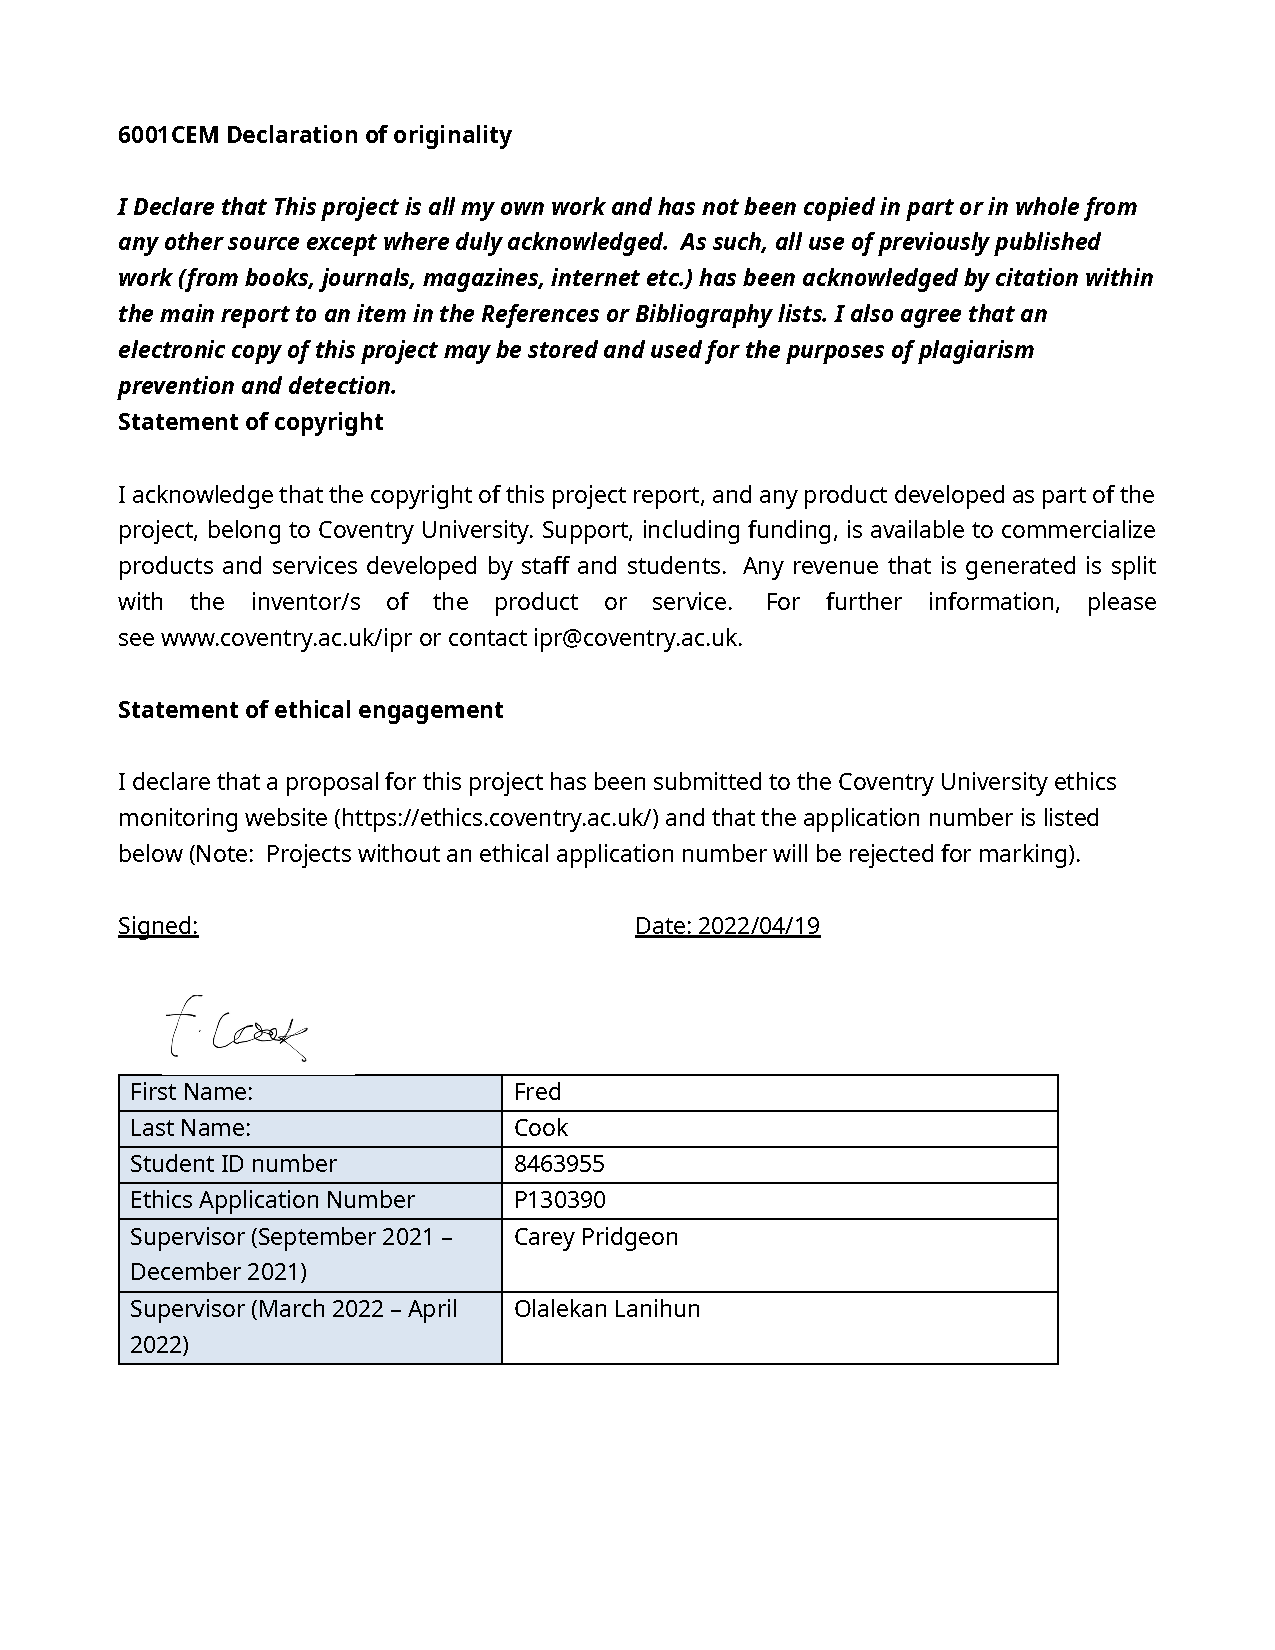
\includepdf{assets/originality-statement.pdf}


\newpage
\tableofcontents
\newpage

\section*{Acknowledgements}
\addcontentsline{toc}{section}{Acknowledgements}
I'd like to thank: Teresa, Stephen, and Lauren Cook, Grace Barnes, and Felix Goodman for their contributions to discussion and support.

\vspace{0.5cm}

I'd also like to thank: Carey Pridgeon, Olalekan Lanihun, and Peter Every for for their guidance and supervision.
\newpage

%\listoftables
\listoffigures
\printglossary[type=\acronymtype, title=List of Acronyms]
\newpage

\pagenumbering{arabic}
\section{Introduction}
C and C++ are famous for their lack of ``safety'', so much so that entire books are written about making them safer, such as John Lakos's 2021 book ``Embracing Modern C++ Safely'' \parencite{cpp-safety-book}. However, as technology becomes more sophisticated, so does the need for the tools used to build said technology. ``Around 70\% of our (Chromium) high severity security bugs are memory unsafety problems (that is, mistakes with C/C++ pointers)'' \parencite{chromium-bugs}; Chromium being the browser engine which is used by Google Chrome, Microsoft Edge, and others (it's worth noting that the chromium developers are now using Rust to improve this \parencite{chromium-rust}). C and C++ have the benefit of having a larger community, more learning resources, and more libraries. They are some of the oldest programming languages still in wide use today \parencite{tiobe-index}, the motivation of this project is therefore to bring some of the benefits of Rust to C++ in order to retain the benefits of both.


%start of literature review

\section{Literature Review}
It's worth noting that sections \ref{subsection:what-is-rust} to section \ref{stages-of-compilation:optimisation} borrow heavily from my own project proposal for that of a similar title, this work can be seen in this paper's literature review \parencite{lit-review}.
\subsection{What is Rust and what makes it different?}\label{subsection:what-is-rust}
Mozilla - the developers of the Rust language say: ``Rust is an open-source systems programming language that focuses on speed, memory safety and parallelism.''  Rust also shares many other similarities with C and C++, these being that they are compiled languages, offer low level control, and (primarily relating to C++) the extensive use of ``Zero cost abstractions'' \parencite{mozilla-rust}.

Rust however aims to go further than it's ``cousin'' languages. The main thing that Rust does to make it ``better'' than languages like C and C++ and set itself apart relates to memory safety. In an interview the initial designer of Rust, Graydon Hoare, says ``Primarily, it's just much safer, less likely to crash.'' when asked ``What makes it (Rust) better than C?'' \parencite{rust-interview}.

Rust offers features not in other languages which allow it to achieve memory safety through guarantees, one of the main methods Rust uses to achieve this is the ``Borrow Checker'' (See section \ref{section:rust-borrow-checker}).
\subsubsection{What is a ``Zero Cost Abstraction?''}
Bjarne Stroustrup (The creator of the C++ language) defines a set of ideals that make C++ what it is, these are: ``A simple and direct mapping to hardware'', and ``Zero-overhead abstraction mechanisms'' making it central to the core philosophy of C++ \parencite{stroustrup-presentation}. Stroustrup goes on to say ``By ``light-weight abstraction'', I mean abstractions that do not impose space or time overheads in excess of what would be imposed by careful hand coding of a particular example of the abstraction.'' \parencite{stroustrup-presentation}. An example of a zero cost abstraction is as follows:

\begin{figure}[H]
	\begin{lstlisting}
#include <array>
int main() {
    std::array<int, 30> myArray;
    myArray.at(25) = 50;
    return myArray.at(25);
}
				\end{lstlisting}
	\caption{``Modern'' C++ std::array zero-cost abstraction}
\label{figure:c++-zero-cost-abstraction}
\end{figure}

This code is trivially simple in that all it does is create a \Colorbox{mygray}{\verb!std::array!} object which is a collection of type \Colorbox{mygray}{\verb!T!}, \Colorbox{mygray}{\verb!T!} in in this case being \Colorbox{mygray}{\verb!int!}, the container is ``wide enough'' for 30 elements. the 26th element is then assigned the value of 50, the program returns the value in the 25th index and terminates.

Similar behaviour can be achieved with traditional, ``hand written'' code as follows:
\begin{figure}[H]
	\begin{lstlisting}[language=c++]
int main() {
    int myArray[30];
    myArray[25] = 50;
    return myArray[25];
}
				\end{lstlisting}
	\caption{Traditional C / C++ array}
\label{figure:c++-traditional-array}
\end{figure}
The behaviour of these two programs is exactly the same and in fact produce the exact same executable, we can see that the assembly output for both using x86-64 \gls{gcca} version 11.2 is as follows

\begin{figure}[H]
	\begin{lstlisting}[language={[x86masm]Assembler}]
main:
        mov     eax, 50
        ret
				\end{lstlisting}
	\caption{Assembly output for figures \ref{figure:c++-zero-cost-abstraction} and \ref{figure:c++-traditional-array}}
	\label{figure:code:assembly-c++-array}
\end{figure}

From this we can see that because these two implementations provide the same assembly output, and therefore same runtime performance as one another. The std::array abstraction has ``zero-overhead'', despite providing the same functionality. In fact it provides more functionality than the traditional C-like implementation, one of these being bounds checking.

For example if we were to try the following and accessing an element out of the range of the container (which would invoke \gls{uba}) which invalidates the program, although it may still run and may produce correct results \parencite{cpp-reference-ub}:

\begin{figure}[H]
	\begin{lstlisting}
#include <array>
int main() {
    std::array<int, 30> myArray;
    myArray.at(25) = 50;
    return myArray.at(100);
}
 	\end{lstlisting}
	\caption{Demonstration of bounds checking with std::array}
\end{figure}

The result of this is a compilation error, this being \Colorbox{mygray}{\verb!terminate called!} \Colorbox{mygray}{\verb!after throwing an instance of std::out_of_range error.!}. This therefore demonstrates that the \Colorbox{mygray}{\verb!std::array!} object provides additional functionality to us, such as the       \Colorbox{mygray}{\verb!std::array<T,N>::at(std::size_t pos)!}   method) which could be hand written, but has little or no advantages in terms of runtime performance to be made.
The argument could be made that the bounds-checking operation could slow down the program, having to check if the index was within the array bounds every time the \Colorbox{mygray}{\verb!at!} method is used, however, because these checks are made at compile-time, there is 0 runtime performance difference, again, demonstrated through the assembly output of the different examples being the same, making the argument moot.

\subsection{Rust and it's relation to C++}
Rust is a relatively new language that aims to remove many of the barriers to entry in the	``systems-level'' programming space \parencite{rust-book1}. Currently the systems-level market is primarily dominated by projects written in C \parencite{embedded-langauges}, so much so that in his article \citetitle{c-language-blog} \citeauthor{c-language-blog} gives a scenario of waking up on an average day, using various appliances in the kitchen, watching the television etc, all of these systems are, according to the author most likely programmed in C \parencite{c-language-blog}.

Graydon Hoare also states that Rust's target audience is ``frustrated C++ developers'' \parencite{rust-interview} and for this reason it's easy to see many of the similarities between the two languages as well as what Rust tries to do different to set it apart from one of the oldest languages still widely in use today, with C++ being the 4th most widely used language in the world at the time of writing according to the TIOBE index, which aims to track the popularity of different programming languages based on metrics such as number of search engine searches in a given time frame and proportion of lines of code written \parencite{tiobe-index}.

\subsection{The Rust Borrow Checker} \label{section:rust-borrow-checker}
The Rust Borrow Checker is a feature in Rust that aims to prevent a series of memory safety mistakes such as ``use after free'' and ``dangling pointers'' without the need for a \gls{gca} \parencite{memory-safety-in-rust}. Because this is done at compile-time, it has no runtime overhead.

A reference in Rust is functionally identical to a reference in C++ which in turn is essentially identical to pointers in C and C++, meaning that to pass a value ``by reference'' means instead to pass the address in memory to that variable. Mutability refers to whether a value can be changed or not, ``mutable'' meaning it can ``mutate'' or change, therefore ``immutable'' meaning it cannot change.

These features being as follows:
\begin{figure}[H]\label{figure:borrow-checker-properties}
\begin{itemize}
    \item{\emph{``That all variables are initialized before they are used.''}}
    \item{\emph{``That you can't move the same value twice.''}}
    \item{\emph{``That you can't move a value while it is borrowed.''}}
    \item{\emph{``That you can't access a place while it is mutably borrowed (except through the reference).''}}
    \item{\emph{``That you can't mutate a place while it is immutably borrowed.''}}
    \item{\emph{``etc''}}
\end{itemize}
\caption{Properties that the rust borrow checker aims to enforce \parencite{borrow-checker-properties}}.
\end{figure}

The rules set out by the borrow checker are:
\begin{itemize}\label{rust:borrow-checker-rules}
    \item{\emph{Any borrow must last for a scope no greater than that of the owner}}
	\item \emph{You may have either but not both of the following:}
	      \begin{itemize}
              \item{\emph{One or more references (\& T) to a resource.} (a T is a type, such as int, character, vector, etc).}
		      \item \emph{Exactly one mutable reference (\& mut T)}
	      \end{itemize}
          \parencite{rust-book}
\end{itemize}

An example of the borrow checker is as follows:

\begin{figure}[H]\label{fig:code:borrow-checker-1}
	\begin{lstlisting}
fn main() {
    let mut x = 5;
    let y = & mut x;

    *y += 1;

    println!("{}", x);
}
 	\end{lstlisting}
	\caption{Demonstration of Rust's borrow checker}
\end{figure}
This program results in an error:
\begin{verbatim}
error: cannot borrow `x` as immutable because it is also borrowed
as mutable
    println!("{}", x);
\end{verbatim}
This happens because we have a ``mutable reference'' to \Colorbox{mygray}{\verb!x!} on line 3, meaning \Colorbox{mygray}{\verb!x!} and \Colorbox{mygray}{\verb!y!} both point to the same place in memory and can both modify the value there. When we then try to pass a reference to \Colorbox{mygray}{\verb!x!} to the \Colorbox{mygray}{\verb!println!!} function meaning we have both, a mutable reference, and a non mutable reference in scope at the same time, violating the rules mentioned in section \ref{rust:borrow-checker-rules}. In this case, the borrow checker prevents a possible race condition in the case that the modifications to \Colorbox{mygray}{\verb!y!} take place in the form of an asynchronous function, such as:
\begin{figure}[H]
	\begin{lstlisting}
use futures::executor::block-on;
async fn increment(x:&mut u32) -> () {
	*num = *num + 1;
}

fn main() {
    let mut x = 5;
    let y = &mut x;

    let future = increment(y);

    println!("{}", x);
    block-on(future);
}
 	\end{lstlisting}
	\caption{Demonstration of Rust's borrow checker with asynchronous function}
\end{figure}
Because of the nature of static analysis being conservative \parencite{ernst-2003-static}, \ref{fig:code:borrow-checker-1} would have no problem executing normally and no race condition would occur, but Rust wants to ensure that if a developer wanted to refactor and make changes later that would have a race condition, minimal structural changes would occur.

This is a common theme in Rust, it forces all code to be correct in all instances.
%\subsection{The need for safety in programming}
%The need for safety in programming has been ignored for a long time. This had lead to a large number of projects that have become part of huge systems we rely on, such as the NHS infrastructure, being bug prone \parencite{cost-of-bugs}. This means that there's economic incentives, aswell as safety reasons to create safe, reliable software.
%
%One example of error prone software causing huge economic damage was \emph{``the CEO of Provident Financial announced a software glitch that led to the company collecting only a little more than half of loan debts on time, the stock prices tumbled 74\% in a single day. The share price reduced from £17.42 to just £4.50. He resigned soon after.''} \parencite{cost-of-bugs}.
%\subsection{Programming language design and implementation}
%\subsubsection{The programming language typing spectrum}
%Programming languages have three criteria (among others) which strongly define it's behaviour. These three features can be plotted on a three-dimensional graph such as in figure the ``Lambda Cube'' (see figure \ref{fig:lambda-cube}). In the Lambda cube the x-axis represents
%
%
%\begin{figure}[H]
%    \begin{center}
%    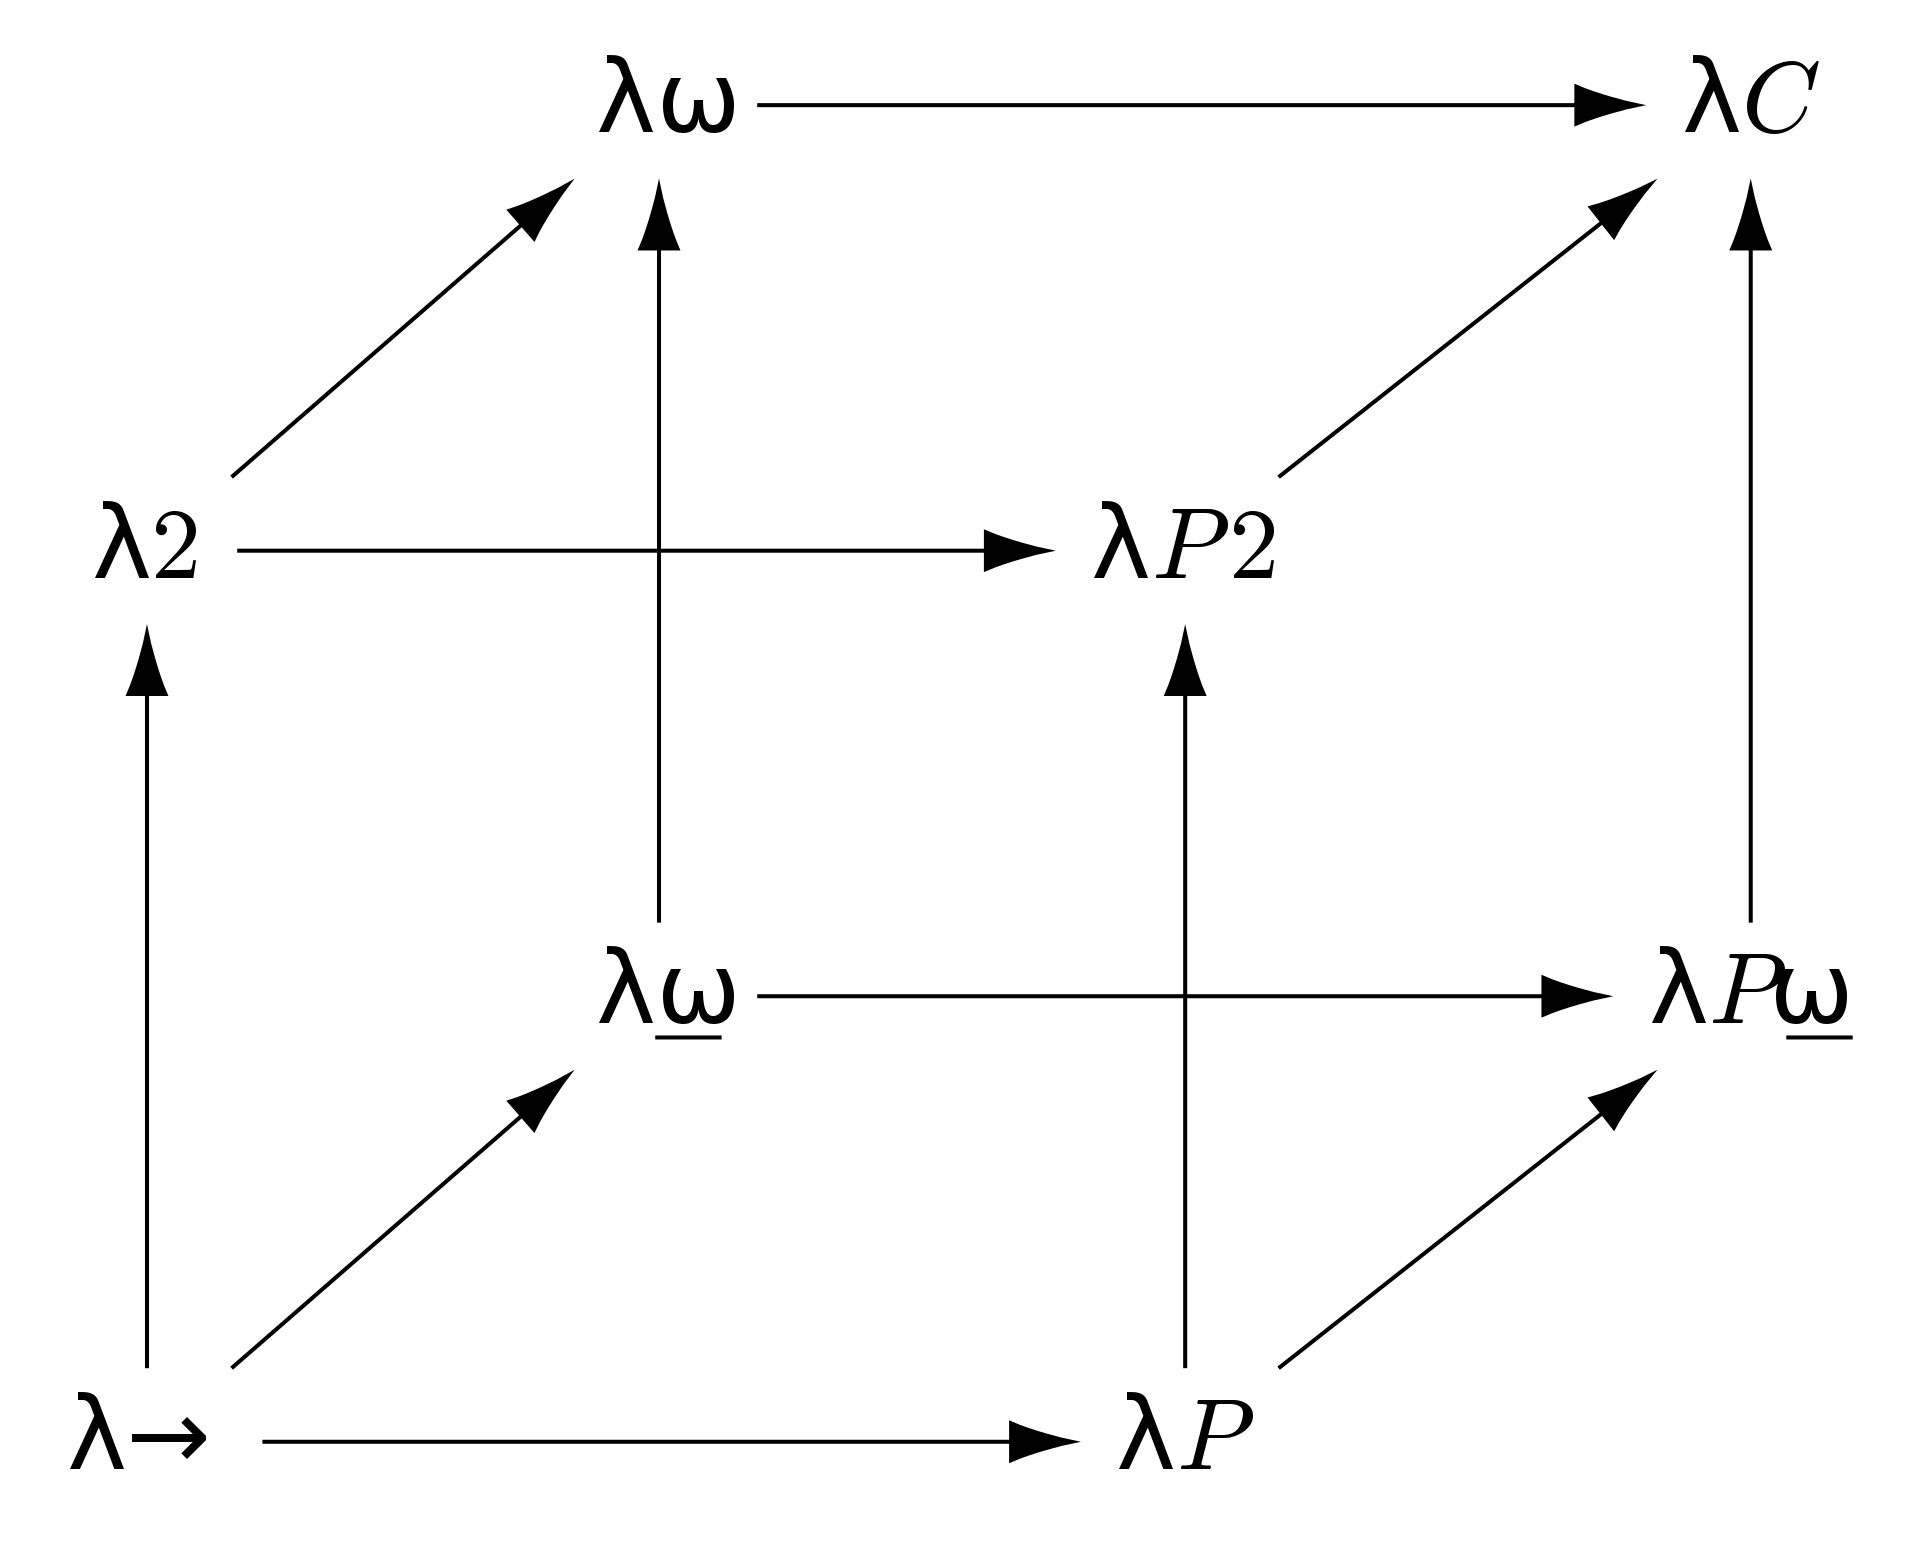
\includegraphics[width=0.4\textwidth]{assets/lambda-cube.png}
%    \caption{Lambda Cube, representing the type system which a programming language implements \parencite{lambda-cube}.}
%	\label{fig:lambda-cube}
%    \end{center}
%\end{figure}
%
%\paragraph{Type-safety}
%\paragraph{Where do other language lay on this spectrum?}

\subsection{Translators, Compilers and Compilation}
Although this paper does not focus on compilers specifically, this knowledge is important as it relates to understanding Rust's implementation of the borrow checker.

Translators are programs which convert source code (plaintext) into executable code.
There are 3 types of translators:
\begin{itemize}
	\item \Glspl{compilerg}
	\item \Glspl{interpreterg}
	\item \Glspl{assemblerg}
\end{itemize}

Each of the three have their advantages and disadvantages, but the most prevalent are \glspl{compilerg} and \glspl{interpreterg}. Compilers generally create faster executing code due to the fact that all the translation is done ahead of time, however, this does mean it can take a long time to start running any given code, interpreters remove this initial wait before execution.

The process of compilation is as follows:
\subsubsection{Lexical analysis}
Lexical analysis is the first stage of compilation and involves taking a stream of input, such as a source code file, and remove all unused pieces of text, such as white space, comments, etc, and output a series of ``Lexemes''. These lexemes essentially representing the smallest pieces of text which represent something. Consider the following code:

\begin{figure}[H]
	\begin{lstlisting}
// beginning of source code
var my-number = 42;
 	\end{lstlisting}
	\caption{Input source code for an example Lexer}
	\label{fig:code:pre-lexer}
\end{figure}

would become a series of lexemes, of \Colorbox{mygray}{\verb!var!}, \Colorbox{mygray}{\verb!my_number!}, \Colorbox{mygray}{\verb!=!}, \Colorbox{mygray}{\verb!42!}, and \Colorbox{mygray}{\verb!;!} \parencite{crafting-interpreters}.

Note that the comment on line 1 is completely removed.

\subsubsection{Symbol Table Construction}
The next stage in the process involves taking the output of the Lexer, and constructing a hierarchical structure (often a \gls{bsta}) which contains information about an identifier (name) such as it’s type, it’s name, it’s scope etc.

\subsubsection{Syntax Analysis}
In Syntax Analysis (also known as ``parsing'') we interpret what the tokens (from the Lexer) mean and check the validity of their structure. For example, in figure \ref{fig:code:pre-lexer}, if the semi-colon were to be removed, the lexer would continue as normal, but the syntax analyser would determine that the program is malformed, because in this language, a semi-colon is needed at the end of every line or it would halt the compilation process.
\subsubsection{Semantic analysis}
Semantic analysis takes a valid series of lexemes from the syntax analyser and checks that they follow the rules of the language. This includes things such as no break statements outside of a loop. The semantic analyser performs other functions as well, such as type checking.

\subsubsection{Code generation}
Code generation could be considered as the final stage of the compilation process (optimisation as described in \ref{stages-of-compilation:optimisation} is optional). It involves generating the executable machine code. Code generators do not produce an executable for interpreted languages such as Python, but do for fully compiled languages such as C.
\subsubsection{Optimisation}\label{stages-of-compilation:optimisation}
Optimisation is an optional stage in the compilation process, which involves the code optimiser indentifying parts of the program which could be replaced with other optimised code. An example of this can be seen in figures \ref{figure:c++-zero-cost-abstraction}, \ref{figure:c++-traditional-array}, and \ref{figure:code:assembly-c++-array} in which the compiler notices that just about all of the code is actually unused and doesn't produce a side effect (something like a write to a file, or anything with persistence) and so it removes it.

\subsection{``Smart Pointers''}
Smart pointers are a way to add additional functionality to pointers (often relating to ensuring safety), such as reference counting. These usually come with additional overhead, such as holding a number in memory to track number of references.

\subsubsection{C++ ``shared\_ptr\textless T\textgreater''}
C++ offers a smart pointer ($shared\_ptr$) which will keep track of how many pointers are pointing to an object, and will only call \Colorbox{mygray}{\verb!free()!} on the memory once there are 0 references to it (implying it is no longer needed).

Because of C++'s \gls{raiia} usage, shared pointers allow for more idiomatic C++ code, more inline with how the rest of C++ is often written \parencite{cppreference-raii}.

Rust offers equivalent for these. Rust's \Colorbox{mygray}{\verb!Rc!} (standing for ``reference count'') for \Colorbox{mygray}{\verb!shared_ptr<T>!}. \Colorbox{mygray}{\verb!unique_ptr<T>!} is not equivalent in Rust, but because of the rules mentioned in section \ref{section:rust-borrow-checker} Rust references act similar to \Colorbox{mygray}{\verb!unique_ptr<T>!}'s most in most cases.
\subsubsection{C++ ``unique\_ptr\textless T\textgreater''}
\Colorbox{mygray}{\verb!unique_ptr<T>!} is similar to a \Colorbox{mygray}{\verb!shared_ptr<T>!} in the sense that it has a reference counter, but \Colorbox{mygray}{\verb!unique_ptr<T>!} only allows for a reference count of 1, and freeing the resource once there are 0 references to it (e.g. the \Colorbox{mygray}{\verb!unique_ptr<T>!} goes out of scope, causing it's destructor to be called).
\subsubsection{Shortcomings of these and how my project relates}
C++'s smart pointers are excellent for improving code safety and allowing for more idiomatic code \parencite{msdocs-smartpointers}. However, C++'s smart pointers do not distinguish between mutable and immutable (or const and non const) references / pointers, instead, treating all these references as the same.

\subsection{The C++ Ecosystem}
As C++ has been around for over 40 years now and has occupied a large space in the programming job market and community, large numbers of tools, standards, etc have been created and maintained over that period of time. This section will give a brief overview of some of the more impactful and most relevant of these.

\subsubsection{Compilers}
The three most popular and widely used compilers in use are \gls{gcca}, Clang, and \gls{msvca}. These have varying levels of conformity with the standards set out by the C++ Standards Committee \parencite{cpp-standard-conformity}.

\gls{gcca} is the oldest of the three, having its 1.0 release in 1987 \parencite{gcc-release} and is published under the GNU General Purpose License and does not have a version compatible with Windows.

Clang is newer and is developed by the \gls{llvma} group, beginning as a research project at the University of Illinois, having its 1.0 release in 2003 \parencite{what-is-llvm}. It's worth noting that as Clang uses the \gls{llvma} ``backend'' for compilation and optimisation this is actually the same as Rust's compiler ``Rustc''.

\gls{msvca} is developed and maintained by Microsoft and had its 1.0 release in 1993 \parencite{msvc-release} and focuses primarily on having full standards compliance, better diagnostics, and code generation / optimisation \parencite{msvc}.

\subsubsection{Tooling}
CMake is one of the most widely used build system generators for C++ projects. CMake is a progression of GNU ``Make'' and in fact generates Makefiles as its standard output (although it is can generate other build system files such as Ninja files). CMake provides a high level interface for automating the process of compiling and linking different files together with libraries, etc.

Valgrind is a project that aims to provide a suite of tools debugging, benchmarking, and analysing C++ programs during runtime. This includes functionality such as analysing memory allocations and usage during the runtime of a program \parencite{valgrind}.

% end literature review

\section{Method}\label{section:method}
\subsection{How Results are Verified and Quantified}
The method for this paper is comprised of creating a series of equivalent (as equivalent as possible) tests in both C++ and Rust. These tests are made to show what is legal and illegal in the two languages with regards to the borrow checker. Other tests are then made to demonstrate the change in a C++ program's behaviour when using my implementation of the borrow checker, and how this new behaviour is more closely aligned to that of an equivalent Rust program. It's worth noting that the Rust based tests are essentially testing whether a file is able to compile, if the file fails to compile then the test passes, this is because it shows that we are catching illegal operations at compile time and therefore preventing runtime errors.

As this is a partial runtime implementation (as opposed to Rust's compile-time implementation) of the borrow checker, the properties that my implementation will provide are points 4 - 5 from figure \ref{figure:borrow-checker-properties}, these relating to having multiple references which can change a value or having references that can read a value while another can change it. This is done through distinguishing between ``const'' and regular or ``non-const'' references to an object. This then ensures that developers are more explicit when declaring regions of code in which these behaviours are desired, and this is more rigidly enforced than in vanilla C++ which assumes the programmer knows what they are doing and gives them a great degree of freedom because of this \parencite{cpp-core-guidelines-talk}.

Tests written in C++ are split into two distinct, separate files; one file \Colorbox{mygray}{\verb!internal_tests.cpp!} contains tests which aim to ensure that the rules of the borrow checker are maintained at all time, and the other file, \Colorbox{mygray}{\verb!test.cpp!} aim to show a series of small scenarios in which this implementation can be useful and prevent unwanted states / behaviours.

\subsection{An Overview of This Implementation}\label{subsection:overview}
The primary method in achieving the goals set out in this paper is as follows: Creating a class which takes a single value as part of its constructor, the type of which does not matter as it is templated code, from now on this paper will refer to the type of the value being held as a \Colorbox{mygray}{\verb!T!} (for example, an instance of \Colorbox{mygray}{\verb!borrow_checked<T>!} holds a \Colorbox{mygray}{\verb!T!}, \Colorbox{mygray}{\verb!T!} representing any type such as \Colorbox{mygray}{\verb!int!}, \Colorbox{mygray}{\verb!string!}, \Colorbox{mygray}{\verb!array<T>!}, etc), this concept is referred to as a ``generic type'' in C++ and Rust as well as other languages. This class is then responsible for encapsulating all functionality associated with reference counting (distinguishing between references which can and which can't change the value held by the class), creating references, etc.

This is done through ``delete''-ing a lot of default operations of the class, such as the copy assignment operator to limit default functionality, such as directly assigning a new value to the object (illegal operation). The object then has an associated states relating to whether it's read only, read / write, or unset, determining what operations can take place on the data held inside, resulting in the program crashing if an illegal operation is made. This choice of removing certain functionality is inspired from \cite{design-philosophy}'s concept of ``defining errors out of existence''.

An important note to make is that in this implementation there is no differentiating between a const reference and a mutable reference, they are the same type of object, however, the methods used to retrieve one of these has a different effect on the internal state of the ``parent'' object, therefore determining legal and illegal operations. Because of the changing of the internal states of the objects it is useful to think of these as different types of references (as mentioned earlier in this subsection), as the internal state of a \Colorbox{mygray}{\verb!const_ref!} is impossible to be present when a \Colorbox{mygray}{\verb!mut_ref!} is also present. Note that \Colorbox{mygray}{\verb!const_ref!} and \Colorbox{mygray}{\verb!mut_ref!} refer to immutable and mutable references (respectively), this naming convention is a combination of C++ and Rust's ``const''-ness declarations, as Rust requires developers to explicitly determine mutability with the \Colorbox{mygray}{\verb!mut!} keyword and inversely C++ requires developers to explicitly declare mutability with the \Colorbox{mygray}{\verb!const!} keyword.

Because the data cannot be written to by all types of references, the data held must be marked as private, and getters / setters used to prevent developers circumventing the methods put in place to prevent unsafe modification of the data.

\section{Evaluation \& Results}
The tests written mentioned in section \ref{section:method} provide a series of scenarios in which the C++ implementation prevents undesired situations which can potentially result in data races (and therefore \gls{uba}). Due to these being tests they can be run with different compiler flags, versions, language standards, etc. to demonstrate that they still work with any configuration the user wishes to use them in. These tests can also be built upon and expanded in the future to demonstrate and test other behaviours.

These tests demonstrate that it is much more difficult to create situations in which data races occur, resulting in an assertion fail in the implementation, and therefore a crash. Due to this being an \Colorbox{mygray}{\verb!assert!} statement as opposed to a \Colorbox{mygray}{\verb!throw!}, it is impossible for the developer to ``catch'' the error and ignore it. This is by design, because, as previously mentioned, data races result in \gls{uba} and therefore ``Renders the entire program meaningless'' \parencite{cpp-reference-ub}. These checks can still be turned off once developers are confident that all code paths are safe in order to reduce runtime overheads and improve performance by using the \Colorbox{mygray}{\verb!#define NDEBUG!} macro (standards compliant) \parencite{ndebug}, the use of \Colorbox{mygray}{\verb!NDEBUG!} also allows the flexibility of incrementally enabling or disabling more instances of borrow checked code for developers.

It's worth noting that some of the tests demonstrating C++ data races seemingly pass or fail at random, this is by design, and due to the nature of data races is effectively the correct behaviour for demonstrating that a data race occurs. All other tests should always pass (and do in the environment and configuration they were written and tested in. The environment in which this code was written and tested in can be seen in appendix \ref{appendix:system-configuration}.

It is also worth noting that despite best efforts, due to limitations of the language which would require significant additional work to fix (which is outside the scope of this project) it's still possible to bypass some of the safety features put in place by this library. This can be done as the \Colorbox{mygray}{\verb!borrow_checked<T>.get_data()!} returns a pointer to the data it holds. This pointer can then be used to manually manipulate data held at the pointer's address (functionality which should be obtained via the \Colorbox{mygray}{\verb!borrow_checked<T>.set_data(T new_data)!} method), therefore essentially always having a mutable reference to the data, regardless of whether other mutable or immutable references exist, this breaks the rules set out by the borrow checker as seen in section \ref{section:rust-borrow-checker}. It should therefore be noted that developers must still take precautions to ensure that their codebase is free of this behaviour, this is an area in which potential future efforts could improve upon.

\section{Discussion}
Other developers are working on bringing similar concepts from Rust that are popular and liked by the community to C++, examples include members from the \gls{llvma} foundation bringing lifetime annotations \parencite{lifetime-annotations-cpp} (which make up another large part of the borrow checker). These ensure that references will never be freed before a use, making it impossible to get a null reference / null pointer error (or undefined behaviour relating to it). This results in performance boost, as a common idiom in C and C++ is to check if a pointer is a ``nullptr'' before reading from it, having a compile time assurance that there will never be a null pointer can greatly improve performance. The C++ Core Guidelines have support for a not\_null smart pointer as part of the Guidelines Support Library which could act as a method to reduce the number of null pointer errors \parencite{cpp-guidelines-notnull}.

While this project is successful at providing an additional option for C++ developers aiming to create safer programs the runtime implementation has a cost of a runtime overhead (which a compile-time implementation, such as Rust's, does not). A compile-time implementation would also offer a greater level of safety, because the one produced as part of this paper only prevents programs getting into states where it is possible to create a data-race, crashing the program when this happens, meaning that in large projects it is possible for potential code paths, which are rarely used, could result in a crash while in production (if not caught by tests). Many academics and developers would say that crashing is preferable to a data race as data races cause \gls{uba} which invalidates the program and the results produced by it \parencite{cpp-reference-ub}. A compile-time implementation offers the safety of having a guarantee that a program will never crash for that reason, increasing developer confidence and lowering cognitive overhead of their codebase. A compile-time implementation was not possible for this paper, as it would require a much longer research and creation process which was not available at the time.

One benefit that a runtime implementation offers that a compile-time implementation does not is compatibility with all compilers. Rust has a single compiler (``rustc'') which acts as an authority for what the Rust programming language is. This offers the benefit of more ``agility'' for Rust - if the community / Rust Foundation decide they want to change something, such as the name of a standard library module, that can be done quickly and without it going through a standards committee, review, publication, etc. as it does for C++, and developers can be sure that the new name is standard. A single compiler also offers a guarantee that code will always compile the same (or much more similar) as there is only one single compiler.

On the other hand, C++ has a written standard \parencite{cpp-standard}, C++ compilers therefore are just programs which aim to conform to these standards as closely as possible with varying degrees of success \parencite{cpp-standard-conformity}. This means that a compile-time implementation would only be compatible with a single compiler, such as GCC, Clang, or MSVC. A runtime-implementation can just be included as a library and used the same across all compilers, allowing for a greater level of adoption.

Another advantage of a runtime implementation is that it offers quicker compile times, compared to a compile-time implementation. Rust is often criticised for having lengthy compile times \parencite{rust-compile-times}, these being longer than that of C++, which is also criticised for long compile times. My implementation brings Rust-like safety at a C++ level of compile-time, making it more suitable for building upon large projects which have already demonstrated, and trust that the majority of their codebase is safe from memory issues and only need to implement extra safety precautions for new code being added. This is due to the fact that my implementation allows for some variables to be reference counted or ``borrow checked'' and others not, allowing developers to fine-tune their safety requirements versus/ runtime performance.

Another possible implementation is that of using inheritance, as opposed to a single class. An inheritance based implementation would see a \Colorbox{mygray}{\verb!borrow_checked<T>!}, along with a virtual (meaning it only acts as a parent class and cannot itself be instantiated) \Colorbox{mygray}{\verb!reference<T>!} parent class, and classes \Colorbox{mygray}{\verb!const_reference<T>!} and \Colorbox{mygray}{\verb!mut_reference<T>!} which inherit from the reference class. This could perhaps be used to provide more compile-time analysis (for example, it's impossible to call a method to change the value held in a \Colorbox{mygray}{\verb!const_reference<T>!} at compile-time) because the method doesn't exist, this would be further more in line with the idea of ``defining errors out of existence'' discussed in section \ref{subsection:overview}.

One issue with this implementation is that it requires values which could normally be stack allocated to instead be heap allocated. This is a problem for a number of reasons such as: reduced capabilities of static analysis and less optimisations on behalf of the compiler leading to fewer errors being caught and optimisations made before runtime, decreased performance due to previously mentioned reasons as well as heap memory in general being slower than stack memory \parencite{stack-vs-heap}, and additionally increased translation unit and binary sizes due to the including of a header file.
Another drawback of this is that it cannot be used to analyse and test existing code without modification. This is due to the fact that the value that we want to have ``borrow checked'' needs to be wrapped in our \Colorbox{mygray}{\verb!borrow_checked!} object first. In order to introduce this to existing code therefore requires changing of function signatures, and replacing code such as $$\Colorbox{mygray}{++x;}$$ with code such as $$\Colorbox{mygray}{x.set\_data(x.get\_data() + 1);}$$ where \Colorbox{mygray}{\verb!x!} is a \Colorbox{mygray}{\verb!mut_ref!}. This also looks worse, and decreases readability of the code, impacting the quality of the codebase for developers, however, in my view this drawback does not outweigh the safety benefits.

Due to the implementation being written in a single header file, this makes it easy for developers to include in any projects they want it for and exclude it in others, it also makes building it easier and prevents potential \gls{abia} issues in the future, which again, are another source of undefined behaviour.

A limitation unrelated to my implementation is the lack of many academic papers. Despite taking information from the most credible sources I could find, these often times still lack the level of peer reviewing and scrutiny that are associated with academic papers. This is a limitation as it contributes to a lower level of research quality and could potentially hinder the quality of this paper. This is due to the fact that there is comparatively little literature surrounding this subject.

\section{Reflection}
\subsection{Scope of The Project}
As demonstrated by my project proposal, my original intent was to create a compile-time version of the Rust borrow checker in C++ (likely for the Clang compiler), however, I learnt overtime that this was not feasible for this paper due to a lack of pre-existing knowledge on this development of compilers and compiler plugins, and a lack of time as this approach would have required a far more substantial amount of programming to be feature complete.

Because of this, it has allowed me to focus on a smaller piece of the larger project of bringing the Rust entire borrow checker to C++.
\subsection{What I've learnt}
This paper has allowed me to explore the Rust programming language's inner workings, and the more theoretical concepts behind it. In addition to this it has furthered my understanding of many C++ related topics such as \gls{uba}, the C++ standards committee and their role, etc. along with more general concepts such as what it means for a program to be ``well defined'', ``thread safe'' etc.

Because of this knowledge it has allowed me to be more confident in my C++ development by ensuring that standards compliant code is used in all places and to take into account the C++ Standards Guidelines where possible.

    \subsection{Project Management}
    Project management primarily consisted of using a Gantt chart to follow how quickly I made progress (see appendix \ref{appendix:gantt}). This allowed me to gauge how quickly I was completing work, and pushed me to estimate how much work was needed for each section. Although the chart was not strictly adhered to at all time, the times when it was (strictly adhered to) allowed me to have enough time to complete the work to a high standard.

    This Gantt chart, in conjunction with a series of meeting notes (see appendix \ref{appendix:meeting-notes}) near the start and end of the project, gave me a strong insight into what research needed to be done for my literature review and how to begin the programming and acted as a way for my supervisor(s) and I to discuss progress, next steps, and concepts relating to this paper. Towards the end of this project these notes acted as a way to ensure that my report and implementation are of a sufficient quality, include all required content (and included no unnecessary content) and allowed me to receive critical feedback over what could be improved about my report.

    During the course of the project my first supervisor left the university, leaving me without a supervisor for a period of time until I was appointed a new supervisor. While this negatively impacted my project as I had perhaps less guidance than I would have had otherwise, the strong guidance in the beginning along with the notes mentioned in appendix \ref{appendix:meeting-notes} meant I had a strong idea of what work was required and the direction my project was heading in.
    \subsection{Potential repercussions}
    \subsubsection{On the C++ Job Market}
    The social implications of this project include the possibility of reduced need for C++ programmers. This is due to the increased safety, maintainability, and debug-ability of codebases which make use of it. This in turn could lead to loss of job / earnings due to a decreased amount of work performed by a team on a C++ codebase as a non-trivial amount is offloaded to the computer, taking away work from a person.

    \subsubsection{On the Rust Community}
    Another potential repercussion is that the continued introduction of Rust features to C++ could reduce potential interest in the project, leading to a slower development, and a slowing of community growth. This is an issue as it is my opinion that Rust offers a superior developer experience, due to a variety of factors (not including the borrow checker) such as superior tooling, compiler analysis, etc, and to slow the progress of this project would be in conflict with my personal support of Rust. However, I recognise that large projects that have been in development for decades with millions of lines of C or C++ code, such as the Linux project, cannot simply move to Rust even if desired. This therefore allows for a small ``bridging'' between the potential future in which Rust completely replaces C++, and today's world in which C++ accounts for large amounts of frequently used codebases (especially when compared to Rust).
%    \subsection{Feedback}
\section{Conclusion}
While this is likely not to be used in production codebases, it acts as an initial method to introducing additional safety concepts perhaps not commonly seen / utilised by C++ developers and can be an educational tool to teach this concept (borrow checking). In addition to this it is possible in the future to build upon this concept and introduce a more robust and compile-time implementation more suitable for fixing legacy code without requiring refactoring of existing code.

In conclusion, while a full implementation would require a larger amount of work and time than my implementation, it seems that there is no reason to think that a full scale implementation of the Rust Borrow Checker in C++ is not possible, and in fact as part of this paper, a partial implementation already exists with other members of the C++ communities working together on creating these solutions \parencite{lifetime-annotations-cpp}.

\newpage

\printbibliography[title=Bibliography, heading=bibintoc]

\section{Appendices}

\appendix
%\begin
    \newpage
    \subsection{Project Management Gantt Chart}\label{appendix:gantt}
\begin{figure}[H]
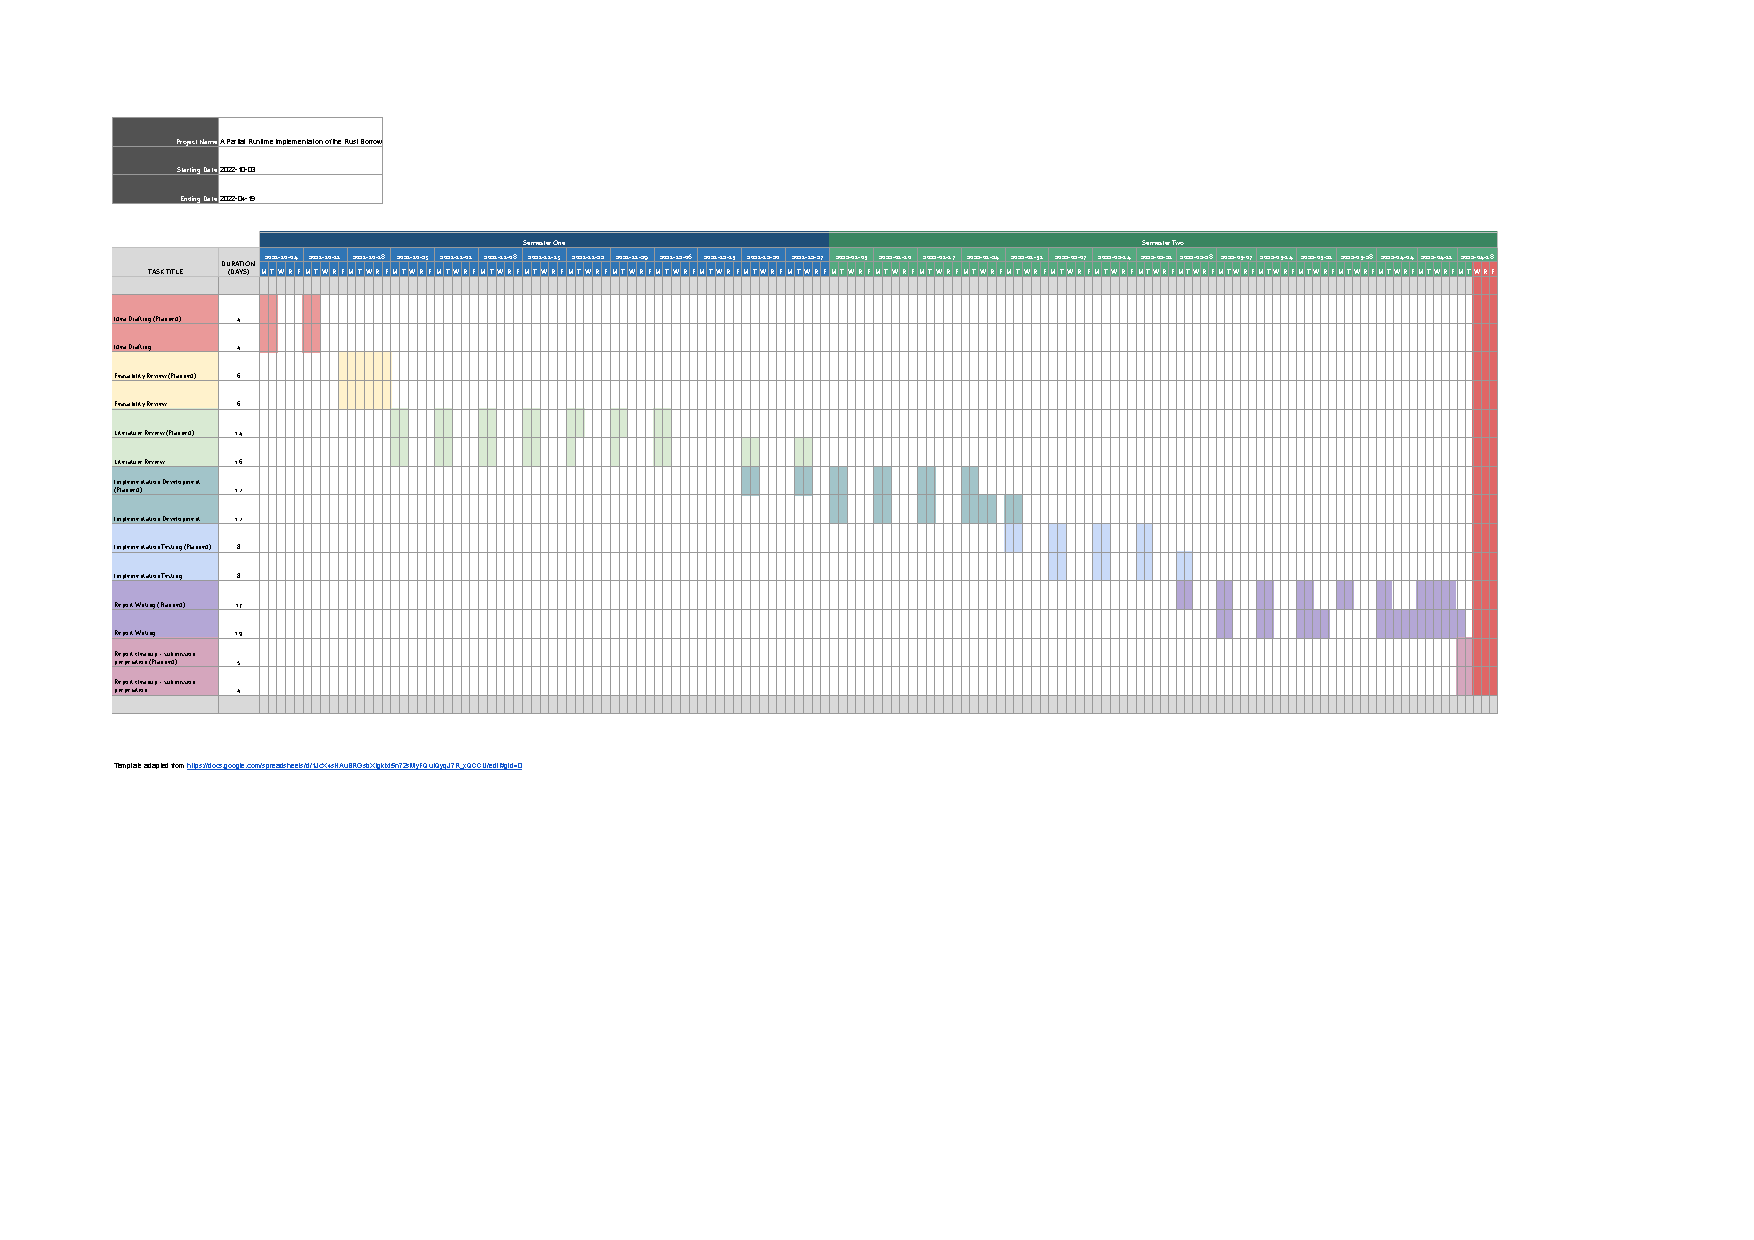
\includepdf[angle=90, scale=0.9]{assets/gantt-chart.pdf}
\end{figure}
%\end{appendices}
\newpage

\subsection{System Configuration}\label{appendix:system-configuration}
\begin{table}[H]
	\centering
	\begin{tabular}{||c | c||}
		\hline
		Variable & Information \\ [0.5ex]
		\hline\hline
		C++ Compiler    & Clang 13.0.1    \\
        \hline
		C++ standard    & 20    \\
        \hline
		CMake version    & 3.22.3    \\
        \hline
		Testing framework    & Google Test Version 1.11.0  \\
        \hline
		Operating system    & Linux (Manjaro) Kernel version 5.10  \\

        \hline
		Rust (Cargo) version    & 1.61.0-nightly  \\

		\hline
	\end{tabular}
\end{table}

\subsection{Meeting Notes}\label{appendix:meeting-notes}
\begin{table}[H]

\hspace*{-6em}
    \begin{tabular}{|| c | m{14cm} ||}
		\hline
		Date & Notes \\ [0.5ex]
		\hline\hline
		01-11-21    & discussed topic\\
                    & spoke about creating a literary review\\
                    &  Advisor gave advice on to go about researching how to potentially implement my project    \\
        \hline
		08-11-21    & discussed literary review as well as literature found \\
                    & Beginning to make my literary review and introduction to paper / topic    \\

        \hline
		15-11-21    & write a paragraph summary for ethics \\
                    & 1500 words for literary review \\

        \hline
		22-11-21    & Discussed progress around literature review \\
                    & Quick overview of literature review / checking of progress \\
                    & Discussed ethics proposal (work to do for next week) \\

        \hline
		29-11-21    & Review of ethics proposal progress \\
                    & for next week: Finish ethics proposal and check again with Carey to check its quality before official submission \\
        \hline
		04-04-22    & Met with new supervisor \\
                    & Discussed topic \\
                    & Discussed current state of report and implementation along with next steps to take \\
                    & Sent current progress and received feedback during the week \\
                    & Discussed avenues to continuing this research outside of academia \\
		\hline
        11-04-22 & Little progress made from last week due to other courseworks \\
                 & Questions about structure of report and required content \\

        \hline
        18-04-22 & Itemize some intro and add research question \\
                 & Mention lacking number of academic sources \\
                 & Add findings to conclusion and reference question \\

        \hline
	\end{tabular}
\end{table}

\subsection{Link to Source Code Repository and Presentation}\label{appendix:source-code}
All source code is stored on a repository on the Coventry Github and can be found at \href{https://github.coventry.ac.uk/cookf2/partial-runtime-rust-borrow-checker-implementation-in-cpp}{https://github.coventry.ac.uk/cookf2/partial-runtime-rust-borrow-checker-implementation-in-cpp}

A short presentation showing usage and brief explanation of the code is also available at \url{https://livecoventryac-my.sharepoint.com/:v:/g/personal/cookf2_uni_coventry_ac_uk/ES4rWczcksFCjXenYXXJ2J8BrMlQcbEOaVLnKrhwvdjTVQ?e=0wbPA2}

Note that if you cannot access this repository or presentattion at the time of viewing please contact me at my university email address of: \href{cookf2@coventry.ac.uk}{cookf2@coventry.ac.uk} or my work email address of: \href{fred.cook.work@gmail.com}{fred.cook.work@gmail.com}

\newpage
\printglossary[type=main]

\end{document}
